% Options for packages loaded elsewhere
\PassOptionsToPackage{unicode}{hyperref}
\PassOptionsToPackage{hyphens}{url}
\PassOptionsToPackage{dvipsnames,svgnames,x11names}{xcolor}
%
\documentclass[
  a4paper,
]{article}

\usepackage{amsmath,amssymb}
\usepackage{setspace}
\usepackage{iftex}
\ifPDFTeX
  \usepackage[T1]{fontenc}
  \usepackage[utf8]{inputenc}
  \usepackage{textcomp} % provide euro and other symbols
\else % if luatex or xetex
  \usepackage{unicode-math}
  \defaultfontfeatures{Scale=MatchLowercase}
  \defaultfontfeatures[\rmfamily]{Ligatures=TeX,Scale=1}
\fi
\usepackage{lmodern}
\ifPDFTeX\else  
    % xetex/luatex font selection
\fi
% Use upquote if available, for straight quotes in verbatim environments
\IfFileExists{upquote.sty}{\usepackage{upquote}}{}
\IfFileExists{microtype.sty}{% use microtype if available
  \usepackage[]{microtype}
  \UseMicrotypeSet[protrusion]{basicmath} % disable protrusion for tt fonts
}{}
\makeatletter
\@ifundefined{KOMAClassName}{% if non-KOMA class
  \IfFileExists{parskip.sty}{%
    \usepackage{parskip}
  }{% else
    \setlength{\parindent}{0pt}
    \setlength{\parskip}{6pt plus 2pt minus 1pt}}
}{% if KOMA class
  \KOMAoptions{parskip=half}}
\makeatother
\usepackage{xcolor}
\setlength{\emergencystretch}{3em} % prevent overfull lines
\setcounter{secnumdepth}{-\maxdimen} % remove section numbering
% Make \paragraph and \subparagraph free-standing
\makeatletter
\ifx\paragraph\undefined\else
  \let\oldparagraph\paragraph
  \renewcommand{\paragraph}{
    \@ifstar
      \xxxParagraphStar
      \xxxParagraphNoStar
  }
  \newcommand{\xxxParagraphStar}[1]{\oldparagraph*{#1}\mbox{}}
  \newcommand{\xxxParagraphNoStar}[1]{\oldparagraph{#1}\mbox{}}
\fi
\ifx\subparagraph\undefined\else
  \let\oldsubparagraph\subparagraph
  \renewcommand{\subparagraph}{
    \@ifstar
      \xxxSubParagraphStar
      \xxxSubParagraphNoStar
  }
  \newcommand{\xxxSubParagraphStar}[1]{\oldsubparagraph*{#1}\mbox{}}
  \newcommand{\xxxSubParagraphNoStar}[1]{\oldsubparagraph{#1}\mbox{}}
\fi
\makeatother


\providecommand{\tightlist}{%
  \setlength{\itemsep}{0pt}\setlength{\parskip}{0pt}}\usepackage{longtable,booktabs,array}
\usepackage{calc} % for calculating minipage widths
% Correct order of tables after \paragraph or \subparagraph
\usepackage{etoolbox}
\makeatletter
\patchcmd\longtable{\par}{\if@noskipsec\mbox{}\fi\par}{}{}
\makeatother
% Allow footnotes in longtable head/foot
\IfFileExists{footnotehyper.sty}{\usepackage{footnotehyper}}{\usepackage{footnote}}
\makesavenoteenv{longtable}
\usepackage{graphicx}
\makeatletter
\def\maxwidth{\ifdim\Gin@nat@width>\linewidth\linewidth\else\Gin@nat@width\fi}
\def\maxheight{\ifdim\Gin@nat@height>\textheight\textheight\else\Gin@nat@height\fi}
\makeatother
% Scale images if necessary, so that they will not overflow the page
% margins by default, and it is still possible to overwrite the defaults
% using explicit options in \includegraphics[width, height, ...]{}
\setkeys{Gin}{width=\maxwidth,height=\maxheight,keepaspectratio}
% Set default figure placement to htbp
\makeatletter
\def\fps@figure{htbp}
\makeatother
% definitions for citeproc citations
\NewDocumentCommand\citeproctext{}{}
\NewDocumentCommand\citeproc{mm}{%
  \begingroup\def\citeproctext{#2}\cite{#1}\endgroup}
\makeatletter
 % allow citations to break across lines
 \let\@cite@ofmt\@firstofone
 % avoid brackets around text for \cite:
 \def\@biblabel#1{}
 \def\@cite#1#2{{#1\if@tempswa , #2\fi}}
\makeatother
\newlength{\cslhangindent}
\setlength{\cslhangindent}{1.5em}
\newlength{\csllabelwidth}
\setlength{\csllabelwidth}{3em}
\newenvironment{CSLReferences}[2] % #1 hanging-indent, #2 entry-spacing
 {\begin{list}{}{%
  \setlength{\itemindent}{0pt}
  \setlength{\leftmargin}{0pt}
  \setlength{\parsep}{0pt}
  % turn on hanging indent if param 1 is 1
  \ifodd #1
   \setlength{\leftmargin}{\cslhangindent}
   \setlength{\itemindent}{-1\cslhangindent}
  \fi
  % set entry spacing
  \setlength{\itemsep}{#2\baselineskip}}}
 {\end{list}}
\usepackage{calc}
\newcommand{\CSLBlock}[1]{\hfill\break\parbox[t]{\linewidth}{\strut\ignorespaces#1\strut}}
\newcommand{\CSLLeftMargin}[1]{\parbox[t]{\csllabelwidth}{\strut#1\strut}}
\newcommand{\CSLRightInline}[1]{\parbox[t]{\linewidth - \csllabelwidth}{\strut#1\strut}}
\newcommand{\CSLIndent}[1]{\hspace{\cslhangindent}#1}

\usepackage{lineno}\linenumbers
\usepackage[scale=0.75]{geometry}
\usepackage[noblocks]{authblk}
\usepackage{lscape}
\usepackage[para]{footmisc}
\usepackage{typearea}

\renewcommand*{\Authsep}{, }
\renewcommand*{\Authand}{, }
\renewcommand*{\Authands}{, }
\renewcommand\Affilfont{\small}
\makeatletter
\@ifpackageloaded{caption}{}{\usepackage{caption}}
\AtBeginDocument{%
\ifdefined\contentsname
  \renewcommand*\contentsname{Table of contents}
\else
  \newcommand\contentsname{Table of contents}
\fi
\ifdefined\listfigurename
  \renewcommand*\listfigurename{List of Figures}
\else
  \newcommand\listfigurename{List of Figures}
\fi
\ifdefined\listtablename
  \renewcommand*\listtablename{List of Tables}
\else
  \newcommand\listtablename{List of Tables}
\fi
\ifdefined\figurename
  \renewcommand*\figurename{Figure}
\else
  \newcommand\figurename{Figure}
\fi
\ifdefined\tablename
  \renewcommand*\tablename{Table}
\else
  \newcommand\tablename{Table}
\fi
}
\@ifpackageloaded{float}{}{\usepackage{float}}
\floatstyle{ruled}
\@ifundefined{c@chapter}{\newfloat{codelisting}{h}{lop}}{\newfloat{codelisting}{h}{lop}[chapter]}
\floatname{codelisting}{Listing}
\newcommand*\listoflistings{\listof{codelisting}{List of Listings}}
\makeatother
\makeatletter
\makeatother
\makeatletter
\@ifpackageloaded{caption}{}{\usepackage{caption}}
\@ifpackageloaded{subcaption}{}{\usepackage{subcaption}}
\makeatother

\ifLuaTeX
  \usepackage{selnolig}  % disable illegal ligatures
\fi
\usepackage{bookmark}

\IfFileExists{xurl.sty}{\usepackage{xurl}}{} % add URL line breaks if available
\urlstyle{same} % disable monospaced font for URLs
\hypersetup{
  pdftitle={Model inner workings - for methods and supplementary sections},
  pdfauthor={Tormey Reimer; Richard S. Cottrell; Alexandra Johne; Sowdamini Sesha Prasad; Marceau Cormery; Gage Clawson; Scott Hadley; Helen Hamilton; Benjamin S. Halpern; Catriona Macleod; Camille White; Julia L. Blanchard},
  colorlinks=true,
  linkcolor={blue},
  filecolor={Maroon},
  citecolor={Blue},
  urlcolor={Blue},
  pdfcreator={LaTeX via pandoc}}


\title{Model inner workings - for methods and supplementary sections}


\author[12]{Tormey Reimer}
\author{Richard S. Cottrell}
\author{Alexandra Johne}
\author{Sowdamini Sesha Prasad}
\author{Marceau Cormery}
\author{Gage Clawson}
\author{Scott Hadley}
\author{Helen Hamilton}
\author{Benjamin S. Halpern}
\author{Catriona Macleod}
\author{Camille White}
\author{Julia L. Blanchard}

\affil[1]{Institute for Marine and Antarctic Studies}
\affil[2]{Centre for Marine Socioecology}


\date{2025-03-26}

\begin{document}
\maketitle


\setstretch{1.15}
\section{Introduction}\label{introduction}

Aquaculture is now the dominant form of aquatic animal food (herein
`seafood') production and is expected to be the primary way we meet
future seafood demand. Freshwater systems will likely continue to
provide the majority of farmed seafood but marine aquaculture is also
poised to expand substantially in numerous areas. Farmed marine fish and
invertebrates are produced near exclusively in coastal waters, and
nearly three quarters of this production is dependent on human-made
feeds. Nearshore locations and feed inputs are necessary to maintain
profitable and productive farming operations but coastal aquaculture
generates a number of challenges. In the crowded coastal zone,
aquaculture operations can conflict with other stakeholder uses such as
recreation, fishing, renewable energy, transport, and tourism. And while
farming marine fish typically generates a far smaller nutrient footprint
than livestock farming, the overt nature of aquaculture in nearshore
regions and evidence of localised nutrient impacts around fish farms
remains a primary public and scientific concern. Identifying strategies
that reduce ecosystem impacts from fish farm waste therefore represents
an important goal for improving marine aquaculture sustainability and
maintaining the sector's social licence to operate.

Aquaculture feeds represent an important lever for reducing nutrient
waste impacts around fish farms. Like all farmed animals, fish and
invertebrates must digest the nutrients contained in feeds before they
can be used for growth. Any nutrients left undigested are egested as
solid waste, and dissolved wastes are excreted as metabolic waste
products. Further, some feed inevitably remains uneaten and is lost to
the surrounding ecosystem. Particulate organic matter (both feed and
faeces) that settles can simplify benthic communities as the oxygen
demand from its decomposition drives the production of sulphides that
kill less mobile faunal, encouraging a lower diversity of opportunistic
scavengers and the growth of bacterial mats (e.g., Beggiatoa spp). Thus,
the chemical composition of the ingredients used in aquaculture feeds
and their digestibility for the farmed species has significant
implications for the nature and reactivity of the waste generate by
marine aquaculture.

. Firstly the overall volume of nutrient waste is dictated by the nature
and intensity of production, that is the farm size, the density of
farmed animals and the feed requirements and efficiency of the species
grown. SecondlDeposition of waste is heavily influenced by water depth
and current speed at the farming site. Once

As farmed fish and invertebrates are fed, whatever

Nutand its impact on marine ecosystems is influenced by many factors.
Farm size Depth Current speed Benthic impact - sediment type/faunal
assemblages/wider marine community High turnover environments - nitrogen
enriched areas Feed influences all of these things

The primary source of organic waste from fed aquaculture production
comes from the excretion and faeces of the farmed animals and through
uneaten feed that dissolves in the water column or settles on the
benthos. The nature and impact of this waste are influenced heavily by
the composition of the feeds fed to farmed animals.

P2 - Waste from aquaculture farms and it's impact is influenced by many
things but the composition of feeds plays a central role. Waste from
aquaculture farms has multiple sources. The primary source of organic
waste comes from the faeces and excretion of the fish or invertebrates.
Uneaten feed produced another key source. The nature and impact of this
waste are influenced heavily by the composition of the feeds fed to
farmed animals Many marine fish are naturally carnivorous so diets used
to be high in fishmeal and oil but increasing fishmeal and oil prices
along with concerns over the sustainability of marine ingredients have
led to a reduction in their use across multiple farmed taxa In lieu of
fishmeal and oil, many plant-based ingredients such as soy protein
concentrate, canola oil, and wheat gluten have replaced them. Changes in
feed composition influences the digestibility of the nutrients held in
each feed and can alter the composition of waste. Of particular concern
are changes (increases) to the presence of reactive nitrogen and
phosphorus in coastal waters that could have an effect on
eutrophication.

P3 Whether or not nutrients lead to eutrophication depends on the
sensitivity of the receiving environment Ecosystems that are already
enriched through natural processes and whose biota is well adapted to
substantial fluxes in available nutrients (e.g.~upwelling zones, dynamic
coastal communities) may be less sensitive while oligotrophic ecosystem
are likely to see considerable changes under nutrient enrichment
scenarios. To understand the impact of aquaculture waste under present
day or future scenarios we need to quantify the volume, nature, and
location of mariculture waste and determine the sensitivity of the
receiving environments to that waste. Yet only recent estimates even
give us the estimated location of marine farms let alone the volume of
nature of the waste produced. To address this gap, we use existing maps
of mariculture location with a bioenergtic model

\section{Temporary questions to
answer:}\label{temporary-questions-to-answer}

\begin{itemize}
\tightlist
\item
  Do the fish reach harvest size within a reasonable amount of time?

  \begin{itemize}
  \tightlist
  \item
    If not, are they growing for the correct amount of time, starting at
    the correct weight?
  \end{itemize}
\item
  Is their FCE/FCR reasonably close to experimental data?
\item
  Is their SGR reasonably close to experimental data?
\end{itemize}

\section{Model approach}\label{model-approach}

We adapted the methods of Baldan et al.
(\citeproc{ref-baldan_r_2018}{2018}) to create a bioenergetic model that
simulates individual growth and farm-scale production for Atlantic
salmon and the resultant nutrient waste in the form of excess labile
nitrogen and phosphorus. The model simulates growth at an individual
level, calculating the change in individual weight through time using:

\[
\frac{dw}{dt} = \frac{A-C}{\epsilon}
\]

Where \(w=\) is wet weight (t), \(t=\) time (d), \(A=\) anabolic rate (J
t\(^{-1}\)), \(C=\) the catabolic rate (J t\(^{-1}\)), \(\epsilon=\)
energy density of body tissues (J t\(^{-1}\)).

Individual models were then upscaled using monte-carlo simulations to
simulate size structure in a population. Size differences were achieved
through different initial starting weights and ingestion rates for
different finfish species. All individuals have a fixed mortality rate
to simulate stocking and harvesting.

\begin{itemize}
\tightlist
\item
  Parameterised for atlantic salmon
\item
  Farms with mean temperature \textless{} 8.5\(^\circ\) were excluded
\end{itemize}

\section{Water temp}\label{water-temp}

Originally, all salmon were transferred to grow-out cages (model began)
on January 1st. This isn't particularly realistic. Now, all farms begin
the modelling period in spring (1st of May in the northern hemisphere,
1st of October in the southern hemisphere).

\begin{figure}

\centering{

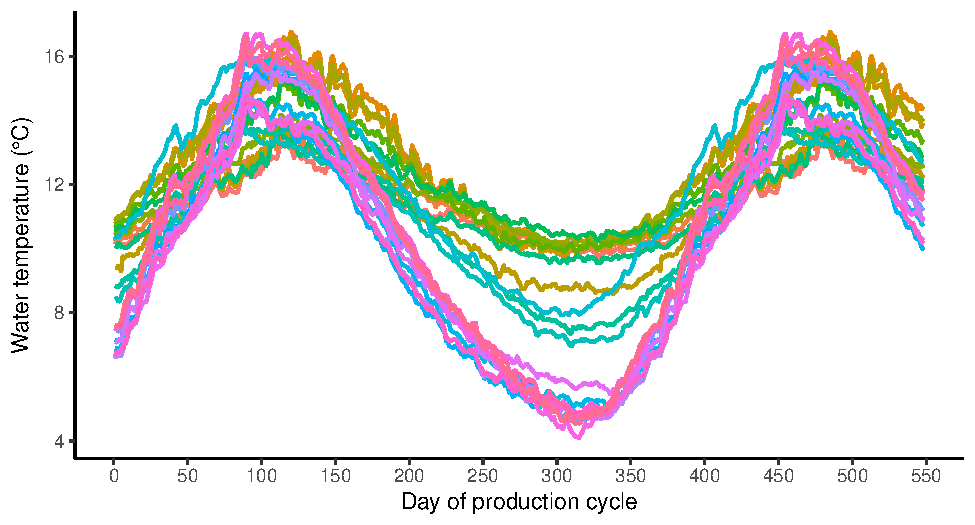
\includegraphics{05_methods_and_supplementaries_files/figure-pdf/fig-water-temp-1.pdf}

}

\caption{\label{fig-water-temp}Water temperature for the production
period, starting at either DOY 121 (1st May, northern hemisphere) or DOY
274 (1st October, southern hemisphere).}

\end{figure}%

\section{Weight}\label{weight}

Figure~\ref{fig-ref-weight} shows the change in weight for 25
individuals grown at different farms. Within the first 5 months
(post-smolt period) the fish grow from 125g to 628.9g, or approximately
5\(\times\) their starting weight. This is better than most production
cycles. By the end of the production cycle (547 days, 18 months) the
fish have grown to a mean of 2027.8 g, and a max of 3110.5 g. This is
not quite what's needed - I'm expecting individual weights to at least
approximate the mean commercial weight of 5kg.

\begin{figure}

\centering{

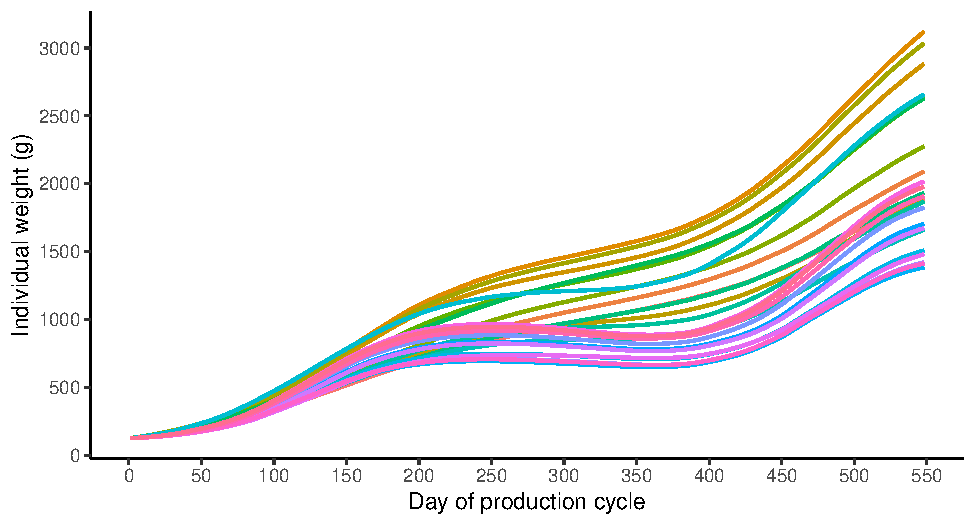
\includegraphics{05_methods_and_supplementaries_files/figure-pdf/fig-ref-weight-1.pdf}

}

\caption{\label{fig-ref-weight}Weight of single individuals grown at 25
random farms across the production period, starting at either DOY 121
(1st May, northern hemisphere) or DOY 274 (1st October, southern
hemisphere).}

\end{figure}%

\begin{figure}

\centering{

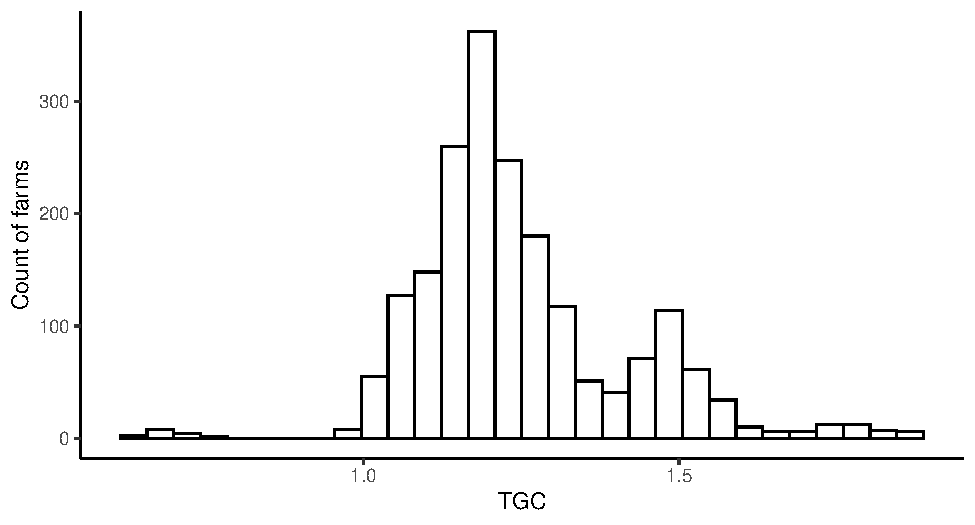
\includegraphics{05_methods_and_supplementaries_files/figure-pdf/fig-ref-TGC-1.pdf}

}

\caption{\label{fig-ref-TGC}Thermal-unit Growth Coefficient (TGC) of all
2721 farms across the production period, starting at either DOY 121 (1st
May, northern hemisphere) or DOY 274 (1st October, southern
hemisphere).}

\end{figure}%

\begin{figure}

\centering{

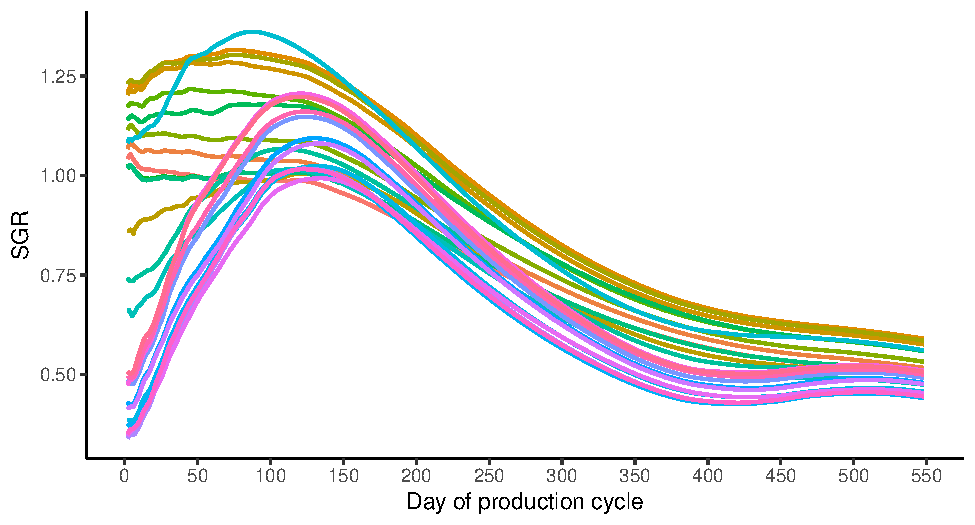
\includegraphics{05_methods_and_supplementaries_files/figure-pdf/fig-ref-SGR-1.pdf}

}

\caption{\label{fig-ref-SGR}Specific growth rate of single individuals
grown at 25 random farms across the production period, starting at
either DOY 121 (1st May, northern hemisphere) or DOY 274 (1st October,
southern hemisphere).}

\end{figure}%

\section{General fish functions}\label{general-fish-functions}

Figure~\ref{fig-functional-response-to-temperature} shows the metabolic
response of all salmon to temperature (affecting their relative
metabolism), and Figure~\ref{fig-feeding-rate-with-temperature} shows
how the salmons' feeding rate changes with temperature.

\begin{figure}

\centering{

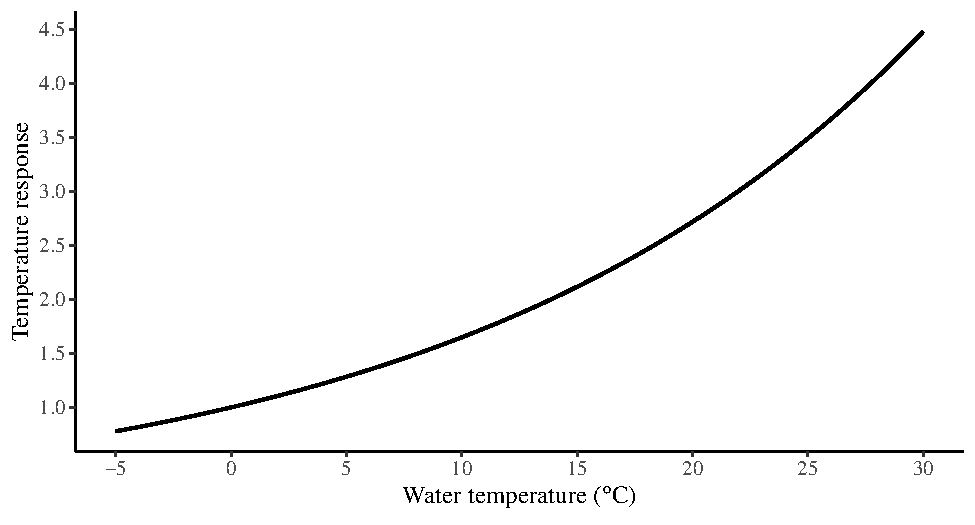
\includegraphics{05_methods_and_supplementaries_files/figure-pdf/fig-functional-response-to-temperature-1.pdf}

}

\caption{\label{fig-functional-response-to-temperature}Metabolic
response of all salmon to temperature within the model.}

\end{figure}%

\[
cat = \epsilon_{O_2} \times k_0 \times T_{resp} \times W^n \times \omega
\]

Relative feeding rate is temperature-dependent and calculated via:

\[
FR_{rel} = e^{b(T_w-T_{opt})} \times \bigg[\frac{T_{max}-T_w}{T_{max}-T_{opt}}\bigg]^{b(T_{max}-T_{opt})}
\]

where \(T_{opt}\) is the optimum feeding temperature, \(T_{max}\) is the
maximum feeding temperature, \(T_w\) is the current water temperature,
and \(b\) is a species-specific shape coefficient.

\begin{figure}

\centering{

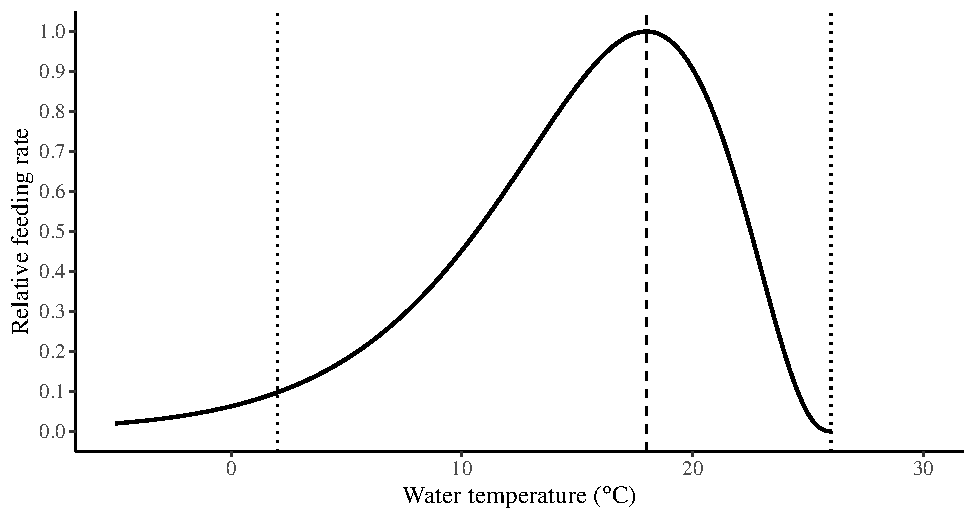
\includegraphics{05_methods_and_supplementaries_files/figure-pdf/fig-feeding-rate-with-temperature-1.pdf}

}

\caption{\label{fig-feeding-rate-with-temperature}Changes in salmons
feeding rate with temperature. The dashed line shows the optimum feeding
temperature for salmon while the dotted lines show the minimum and
maximum feeding temperatures.}

\end{figure}%

\section{Feed data}\label{feed-data}

Incorporated the individual digestibility of each ingredient and
switched to tracking ingredients separately instead of feed -- this
unfortunately makes the model run slower but I think it will be worth it
once the digestibility coefficients from the experiments are
incorporated.

\section{Individual runs}\label{individual-runs}

I set up some ``example fish'' to speed up future model adjustments --
basically fish that are the average of their whole farm, easier than
running 5000 fish per farm while I'm making changes.

\subsection{Food provided vs food
eaten}\label{food-provided-vs-food-eaten}

Within the model, salmon have a maximum ingestion potential (based on
their weight and individualised feeding rate). The actual food ingested
is 97\% of their ingestion potential (food encounter efficiency) or the
total food provided, whichever is less.
Figure~\ref{fig-food-prov-theoretical} shows an example of how food
provided scales with potential individual ingestion.

\begin{figure}

\centering{

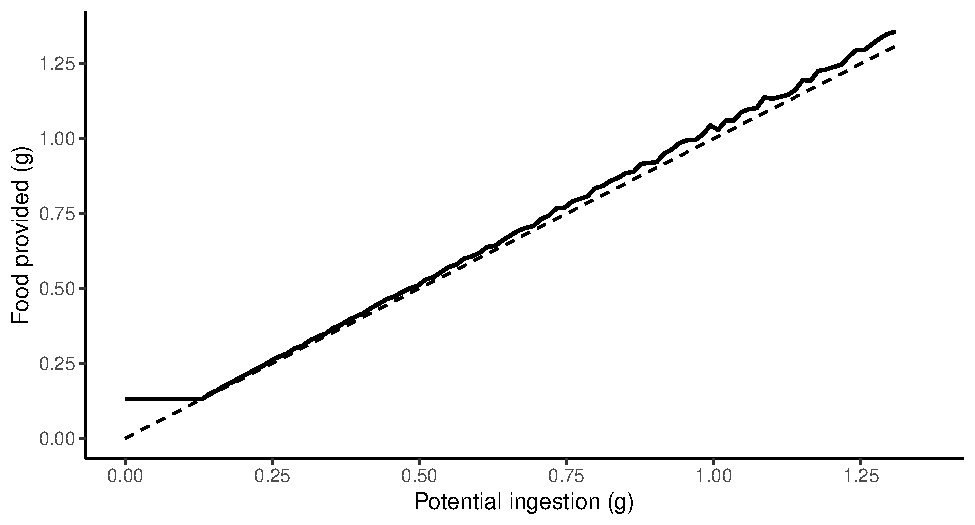
\includegraphics{05_methods_and_supplementaries_files/figure-pdf/fig-food-prov-theoretical-1.pdf}

}

\caption{\label{fig-food-prov-theoretical}Example of food provided based
on potential ingestion (where feeding rate ranges from 0 to 1). This
curve is constructed with a single fish of mean starting weight (125 g)
and average maximum ingestion rate (0.035). The dashed line shows food
provision == potential ingestion.}

\end{figure}%

Therefore, uneaten feed can be quite high (up to \textasciitilde30\%)
when relative feeding is \$\leq\$10\%. But generally, the median amount
of uneaten food is 3.4\% (Figure~\ref{fig-uneaten-feed}).

\begin{figure}

\centering{

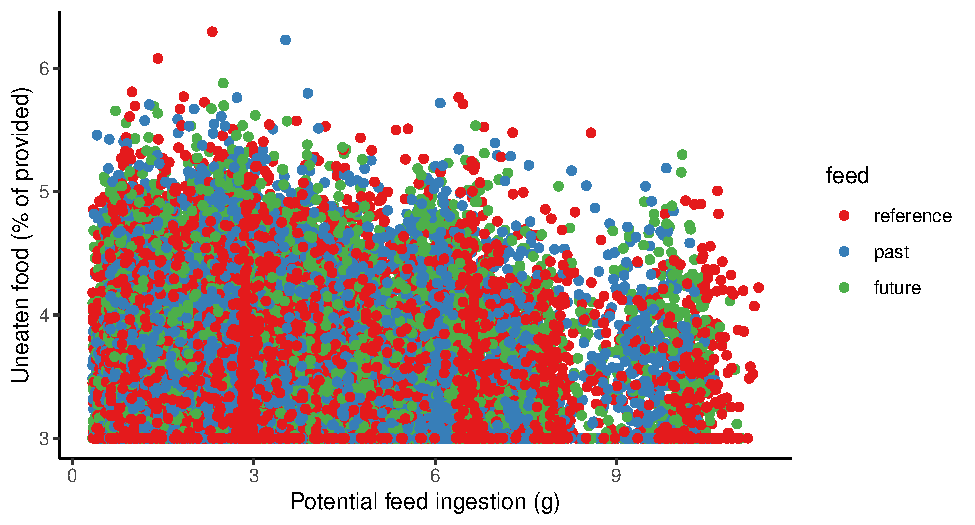
\includegraphics{05_methods_and_supplementaries_files/figure-pdf/fig-uneaten-feed-1.pdf}

}

\caption{\label{fig-uneaten-feed}Difference between food provided and
actual ingestion (i.e.~total food ingestion efficiency) for 25 random
farms.}

\end{figure}%

\section*{References}\label{references}
\addcontentsline{toc}{section}{References}

\phantomsection\label{refs}
\begin{CSLReferences}{1}{0}
\bibitem[\citeproctext]{ref-baldan_r_2018}
Baldan, Damiano, Erika Maria Diletta Porporato, Roberto Pastres, and
Daniele Brigolin. 2018. {``An {R} Package for Simulating Growth and
Organic Wastage in Aquaculture Farms in Response to Environmental
Conditions and Husbandry Practices.''} \emph{PLOS ONE} 13 (5): e0195732.
\url{https://doi.org/10.1371/journal.pone.0195732}.

\end{CSLReferences}




\end{document}
